% ============================================================================
\section{Introduction}\label{sec:intro}

% ============================================================================

Cookie banners run by consent-management platforms (CMPs) have spread across the web \citep{degeling2019value,hils2020emergence,kretschmer2021cookie,jha2025cmp} and act as access control over third-party code: a CMP's script blocker holds back listed vendors' tags until the visitor agrees, but only in the page's main document, not in web workers or sandboxed iframes \citep{whatwg_html}. On Shopify, which hosts millions of stores \citep{assabese2026shopifyapps}, most app pixels and all custom pixels run in such sandboxes, gated only by Shopify's consent state \citep{shopify_aboutpixels,shopify_pixelprivacy,shopify_customerprivacy}; since 26 August 2026 they have also replaced retired scripts on every plan's order-status and thank-you pages \citep{shopify_checkout_upgrade}. \storeC, an anonymized store that a YouTube creator links to with a code naming each video, lists TikTok's pixel script in its consent tool's blocklist, yet TikTok's pixel sent the landing URL, code included, to TikTok from a web worker while the banner still waited (Fig.~\ref{fig:situating}a). The blocklist said ``blocked''; the pixel sent the code anyway. We measure how often consent is lost this way, where, and whether visitors' choices repair it, on popular Shopify stores visited from California.

\begin{widefig}
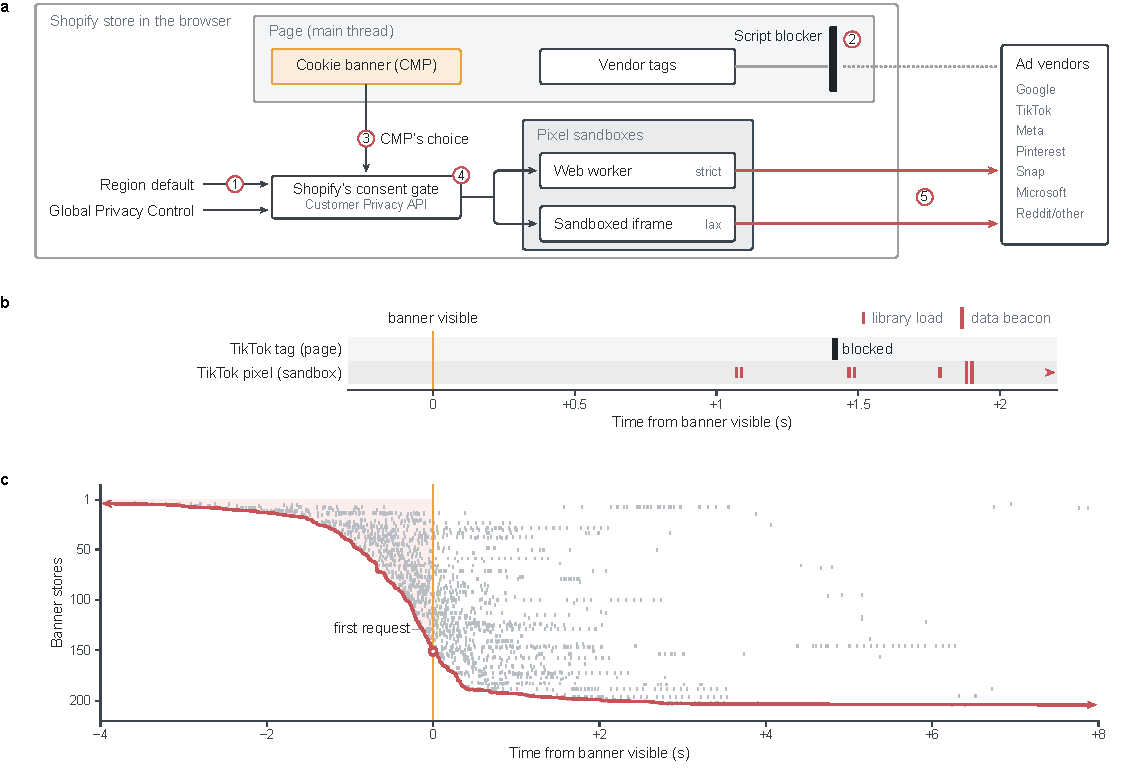
\includegraphics{fig1.pdf}
% GENERATED by paper/integrate_figures_v2.py from figures/v7/fig1/caption_fig1.tex (v2 figure caption, rendered by the figure script).
% Do not edit: change the figure script and re-run build.sh.
\caption{\textbf{Consent is lost at five points between the cookie banner and Shopify's sandboxed pixels.}
(a)~A Shopify store in the browser (outer frame), drawn as nested regions. Top: the page's main thread (light grey ground), where a consent-management platform's (CMP) cookie banner (amber, the colour of its appearance in b and c) and its script blocker (black wall) run; the blocker stops vendor tags in the page (grey line; dotted: the path it cuts). Bottom: Shopify's Web Pixels Manager starts each app or custom pixel in a sandbox isolated from the page (pixel sandboxes, darker grey ground), a web worker (strict runtime) or a sandboxed iframe (lax runtime), once Shopify's consent gate (its Customer Privacy API) allows every purpose that the pixel declares. The gate is set by the store's region default, by the CMP's choice if the CMP writes it to Shopify, and by Global Privacy Control (GPC). The sandboxes stand under the page's vendor tags (the same vendors' code, isolated), and the pixels' requests (brick arrows) leave the browser for the ad vendors underneath the blocker, which covers the page only; the ad-vendor box lists the vendor groups used in every figure. Consent is lost at five of the drawn elements, marked in a by outlined numerals: (1)~the region default, `allowed until choice' on 1,103 of 1,349 stores that returned one (Methods; Fig.~3 measures its effect); (2)~the script blocker (blocked on paper): it cannot see into the sandboxes, so on 46 of 89 stores (51.7\%; Wilson 95\% confidence interval (CI) 41.5--61.8\%) whose CMP listed an ad vendor as blocked and wrote no `yes' to Shopify, that vendor fired from the sandbox anyway in the Default load (no click; main and lower-ranked expansion samples combined; Fig.~4); (3)~the CMP's choice, which arrives late: in loads where a CMP wrote `marketing: no' without a click, 525 of 535 third-party sandboxes that declare marketing had already started (Fig.~5c); (4)~the consent gate, which reads declared purposes only: under GPC, a pixel that declares no purpose fired on 191 of 1,354 stores where Shopify set `sale of data: no' (Fig.~S8c; Fig.~5b counts each store in one class only); (5)~the path to the vendors, which a refusal does not cut: after a Decline (a click on the banner's reject button), a pixel that declares the refused purpose kept sending (same page or unload beacons) on 32 of 196 stores with a recorded refusal (Fig.~5b).
(b)~Point (2) in one page load (re-check, no click). The store is from the main sample; its CMP (Pandectes) lists TikTok as blocked and wrote no `yes'. It is the first by ID among the 5 stores where the blocker neutralized a declared-blocked vendor's page tag while that vendor's sandboxed pixel sent requests, and of its two such vendors TikTok sent more sandboxed requests. The axis is time from the banner becoming visible (amber line), which happened 1.3~s after navigation start; the times below are from navigation start, and no choice was made. The two rows repeat a's grounds (light grey: the page; darker grey: the sandbox). Top row: the blocker neutralized TikTok's tag as it was inserted, at 2.7~s (black bar, the wall of a; script type `javascript/blocked'); the tag sent no request. Bottom row: TikTok's pixel in a sandboxed iframe, which had requested its library 0.34~s earlier, sent 5 library loads (short brick ticks; key above the axis) and 2 data beacons (tall brick ticks) between 2.4 and 3.2~s, and 1 more beacon at 13.2~s (arrowhead at the right end of the row); requests of one kind less than 50~ms apart are drawn side by side. This axis has a larger scale than that of (c); the two zeros are aligned.
(c)~The same failure at scale: every banner store whose sandboxed pixel sent an ad request before any choice (205 of 409 stores that showed a banner), one row each, sorted by its first sandboxed ad request (brick line) and timed from the banner becoming visible (amber line; the detector polls every 250~ms). Grey ticks: the stores' sandboxed ad requests in the Default load; the 55 requests earlier than the axis and the 68 later are not drawn, and the brick line leaves the axis (arrowheads) for the 4 stores whose first request came earlier and the 1 whose first request came later. Rows above the point where the brick line crosses the amber line (open circle; the pale brick ground between the two lines is the time before the banner): the 151 of 205 stores (73.7\%; Wilson 95\% CI 67.2--79.2\%) whose first request came before the banner (Fig.~S6b). Per vendor group: Fig.~S6a; per-store request counts: Fig.~S6e.
All loads from one residential vantage point in California, USA; main sample: 1,358 popular Shopify stores from the Tranco top 200,000.
Panel~(a): Drawn by figure-generation scripts written with AI assistance (Section~\ref{sec:method-ai}).}
\label{fig:situating}

\end{widefig}

Consent measurement has examined banners and what they record: their dark patterns \citep{nouwens2020dark,berens2024cookie} and, in declared-versus-observed audits, consent strings \citep{matte2020banners}, cookie declarations \citep{bollinger2022automating} and consent data \citep{zhang2024cschecker} against observed behaviour. Tracking before a choice or after a rejection is common \citep{papadogiannakis2021post,martinez2022compliance,bouhoula2024automated,martinez2025million}, and rejection and the Global Privacy Control (GPC) signal each remove only part of the tracking cookies \citep{rasaii2025intractable}. US studies have read GPC compliance from privacy strings \citep{zimmeck2023gpc,hausladen2025gpc} and followed opt-outs into advertising systems \citep{liu2024opted,aziz2024johnny}; root-cause studies locate CMP failures in configuration and scanning \citep{tang2025navigating,toth2022dark}. Most such studies audit consent at the banner, in cookies or in consent strings, treating the CMP as the enforcement point.

Where third-party code runs has been studied separately: sandboxes were built to protect a host page from embedded code \citep{terlouw2010adjail,ingram2012treehouse}, trackers slip past users' blockers \citep{bashir2018websockets,dimova2021cname,chen2021filterlist,bottger2026fpt}, and tags under Google Tag Manager's consent layer can leak data \citep{mertens2025gtm}. For Shopify, the one academic consent study we found assessed its native banner \citep{nouwens2025crosscountry}, while the platform, CMP vendors and practitioners document the sandbox, its permissive regional default, blockers that cannot reach app pixels, and pixels that fire before the consent state is set \citep{shopify_aboutpixels,shopify_customerprivacy,truevault_apppixel,onetrust_ecommerce,pandectes_blocking,analyticsninja2025pixels,weltpixel2026race}. Consent audits show what was decided or collected, not which component let the code run; to our knowledge, none fully attributes vendor requests to their execution context and joins them to the platform gate that started their code (Section~\ref{sec:related}). The mechanism is documented, so we claim not its discovery but, to our knowledge, the first measurement of its consequences across stores.

We treat consent as an access-control policy with two enforcement points (Section~\ref{sec:bg-threat}), the CMP's blocker for tags in the main document and Shopify's gate for sandboxed pixels, and lost consent as a request that passes both against the stated policy, a failure of complete mediation \citep{saltzer1975protection}. Our crawler attaches to the page and every worker and iframe, attributes each ad request to its execution context, and joins sandboxed requests to the pixel's declared purposes, Shopify's consent state and the sandbox's start (Fig.~\ref{fig:methods}); comparing these requests with CMP blocklists extends declared-versus-observed auditing \citep{matte2020banners,bollinger2022automating} to execution contexts. This separates a blind blocker from an open or late gate and from a pixel that declared nothing, which cookie-based audits and unattributed network crawls cannot (Section~\ref{sec:disc-beyond}). We load each store with no click (\emph{Default}), a reject click (\emph{Decline}) and GPC, and ask four research questions:
\begin{itemize}
  \item[\RQ{1}] \emph{Before any choice.} On banner stores, how often do sandboxed ad pixels fire before a choice, and with what is this associated?
  \item[\RQ{2}] \emph{Blocked on paper.} When a blocklist, a message to Shopify or the region setting says ``no'' before any choice, how often does a sandboxed pixel fire anyway?
  \item[\RQ{3}] \emph{Choices.} Do Decline and GPC stop sandboxed pixels, and through which path?
  \item[\RQ{4}] \emph{Reach.} What reaches vendors through the requests not stopped?
\end{itemize}
As validation, we test stability and agreement with native GPC.

We loaded 1,358 Shopify storefronts from the Tranco top 200,000 \citep{lepochat2019tranco,tranco_L5PZ4} and 34 creator-linked stores from one residential connection in California; a second crawl added 116 stores from Tranco ranks 200,001--1,000,000 chosen for their CMP blocklists, and piloted Wix, BigCommerce and first-party tag gateways. We find four things. First, before any choice, sandboxed ad pixels fired on 70.2\% of banner stores whose region default allowed tracking and on 24.0\% where it denied it, a gap that held within consent products (Fig.~\ref{fig:region-default}). Second, on 46 of 89 blocklist stores whose CMP had not itself consented, a vendor the blocklist declared blocked fired from the sandbox before any choice, and blocklist stores fired more often than comparable stores, not less (Fig.~\ref{fig:blocked-on-paper}). Third, Shopify's gate held back 2,206 of 2,234 marketing pixels under a denying default, but consent was lost around it: automatic ``no'' writes came after 525 of 535 third-party marketing sandboxes had started, a new sandbox still sent ad requests after a working Decline on 22.9\% of stores, and 34.7\% of stores with sandboxed requests kept sending them under GPC (Fig.~\ref{fig:choices}). Fourth, 63.4\% of sandboxed ad beacons in the Default load carried the full landing URL, query string included (Fig.~\ref{fig:reach}). We also contribute a reusable gate audit, a taxonomy of 24 consent products' Shopify integrations (Table~\ref{tab:cmp-modes}), the pilot (Section~\ref{sec:res-beyond}), fixes, and ConsentCheck, a merchant self-test (Section~\ref{sec:discussion}).
